% chktex-file -1
% chktex-file 24
% chktex-file 9
\chapter{Method}

\fxerror{Introduction to chapter.}

\section{Hidden Markov Models}

\fxerror{Write a better introduction to HMM's.}

In the section the definition of and notation for a Hidden Markov Model and the
Viterbi algorithm will be presented using the notation also used by
\citet{sand2013ziphmmlib}.

A hidden Markov model is a statistical model in which it is assumed that an
observed sequence is generated by a Markov process with unobserved hidden
states. Hence, for a sequence $Y_{1:T} = y_1y_2\dots{}y_T \in \mathcal{O^*}$
generated by the model there exist one or more hidden sequences
$X_{1:T} = x_1x_2\dots{}x_T \in \mathcal{H^*}$, with $\mathcal{O}$ and
$\mathcal{H}$ being finite alphabets over the observables and hidden
states. The hidden sequence may be seen as a explanation of the observed
sequence.

Formally a HMM can be defined as
\begin{itemize}
\item $\mathcal{H} = {h_1, h_2, \dots, h_N}$, a finite alphabet of hidden
  states;
\item $\mathcal{O} = {o_1, o_2, \dots, o_M}$, a finite alphabet of observables;
\item a vector $\Pi = {(\pi_i)}_{1 \le i \le N}$, where $\pi_i = \Pr(x_1 =
  h_i)$ is the probability of the model starting in hidden state $h_i$;
\item a matrix $A = {\{a_{ij}\}}_{1 \le i \le N}$, where $a_{ij} = \Pr(x_t
  = h_j \mid x_{t - 1} = h_i)$ is the probability of a transition from state
  $h_i$ to state $h_j$;
\item a matrix $B = {\{b_{ij}\}}_{1 \le i \le N}^{1 \le j \le M}$, where
  $b_{ij} = \Pr(y_t = o_j \mid x_t = h_i)$ is the probability of state
  $h_i$ emitting $o_j$.
\end{itemize}

A HMM is parametrized by $\pi$, $A$, and $B$, which is denoted by $\lambda =
(\pi, A, B)$.

\section{The Classical Viterbi Algorithm}
\label{sec:class-viterbi-algor}

The Viterbi algorithm finds the probability of the most likely sequence of
hidden states given a model $\lambda$ and an observed sequence $Y_{1:T}$ by
maximizing the probability of the observed and hidden sequences for all
possible hidden sequences: $\Pr(Y_{1:T} \mid \lambda) = \max_{x_{1:T}}
\Pr(Y_{1:T}, X_{1:T} = x_{1:T} \mid \lambda)$. This may be computed efficiently
by filling out a table, $\omega$, with entries $\omega_t(x_t) = \Pr(Y_{1:t},
X_t = x_t \mid \lambda) = \max_{x_{1:t-1}} \Pr(Y_{1:t}, X_{1:t} = x_{1:t} \mid
\lambda)$ column by column from left to right, using the recursion
\begin{equation}
  \label{eq:1}
  \begin{aligned}
    \omega_1(x_1) &= \pi_{x_1} b_{x_1, y_1} \\
    \omega_t(x_t) &= b_{x_t, y_t} \max_{x_{t - 1}} \omega_{t - 1}(x_{t - 1})
    a_{x_{t - 1}, x_t}.
  \end{aligned}
\end{equation}
After filling out $\omega$, $\Pr(Y_{1:T} \mid \lambda)$ can be computed as
$\Pr(Y_{1:T} \mid \lambda) = \max_{x_T} \omega_T(x_T)$.

Note that only the last filled out column of $\omega$ needs to be stored, since
the recursion in equation~\eqref{eq:1} only needs the previous column to
compute the new one. Hence, the space consumption of the algorithm will be the
space needed for two columns and the input sequence, that is $O(N + T)$. To
fill out a cell in $\omega$ Viterbi maximizes over all cells in the previous
column resulting in a running time of $O(N^2 T)$.

\subsubsection{Backtracking}
\label{sec:backtracking-1}

To obtain the most likely sequence of hidden states corresponding to the
likelihood, $X_{1:T}^* = x_1^*, x_2^*, \dots, x_T^*$, also known as the
\emph{Viterbi path}, another table of the same size as $\omega$ is stored with
pointers from each state in a column to the maximizing previous state. When the
last column has been computed in $\omega$, the last state in the Viterbi path
may be found using $x_T^* = \argmax_{x_T} \omega_T(x_T)$. From this state the entire
path can be found by following the pointers in the table.

The space consumption of this backtracking algorithm is the size of $\omega$
which is $O(N T)$. Backtracking is done in $O(T)$ time using the table of pointers.

A space consumption of $O(N T)$ might be a problem in some scenarios. Another
way to backtrack is described by \citet{Tarnas01061998}. By using this approach
the space consumption can be reduced to $O(N \sqrt{T})$ while the assymptotic
running time of the algorithm is preserved.

Instead of storing the entire $\omega$ table in memory only the last column of
blocks of some size $B$ is stored. These columns may be called checkpoints. A
table of pointers corresponding to a block can be recomputed using the
checkpoint of the previous block, since computing a column only requires the
previous block as seen in equation~(\ref{eq:1}). When backtracking $x_T^*$ may
be found as described above. The pointer tables are recomputed one at a time
for each block from right to left. When a table for a block has been recomputed
it is backtracked. Hence, only one block is kept in memory at a time. If
$B = \sqrt{T}$ is chosen, the space consumption of this algorithm is
$O(N \sqrt{T})$. The Viterbi computations are now done two times, so the
algorithm will be a bit slower, but it keeps having the same assymptotic
running time of $O(N^2 T)$.

\section{Viterbi as Linear Algebra}
\label{sec:algorithm-as-linear}

In this chapter the theory of making the Viterbi algorithm faster by exploring
repetitions is discussed. First, the algorithm is reformulated into matrix
operations; second, the use of byte pair encoding is explained; and finally
a solution to make the computation numerically stable is explained.

The above classical Viterbi algorithm can be reformulated into a number of
matrix multiplications. This is what \citet{sand2013ziphmmlib} and
\citet{lifshits2009speeding} use too. First, let $B_{o_i}$ be the diagonal
matrix, having the emission probabilities of $o_i$ of the diagonal:
\begin{equation*}
  B_{o_i} =
  \begin{bmatrix}
    b_{1, o_i} &            &        &            \\
               & b_{2, o_i} &        &            \\
               &            & \cdots &            \\
               &            &        & b_{N, o_i} \\
  \end{bmatrix}
\end{equation*}
and let
\begin{align*}
  C_{o_i} &= B_{o_i} A^* \\
  C_1 &= B_{y_1} \pi,
\end{align*}
where $A^*$ is the transpose of $A$.

Now $\omega_t$ can be computed using $C_{y_t}$ and $\omega_{t - 1}$ as
\begin{equation}
  \label{eq:2}
  \omega_t = C_{y_t} \odot \omega_{t - 1} = C_{y_t} \odot C_{y_{t-1}} \odot
  \dots \odot C_1,
\end{equation}
where $\odot$ is the max-times matrix multiplication defined as ${(A \odot
  B)}_{ij} = \max_k A_{ik} \cdot B_{kj}$.

The classical Viterbi algorithm corresponds to computing this from right to
left, but since matrix multiplication and max-times matrix multiplication is
associative the product may be computed in any order.

Backtracking is achieved in the same way as for the classical Viterbi algorithm
as described in section~\ref{sec:class-viterbi-algor}.

The space consumption and running time of this algorithm has changed, compared
to the classical Viterbi algorithm. For each symbol $o_i$ in the alphabet of
observables the corresponding matrix $B_{o_i}$ is created, thus requiring
$O(M N^2)$ space. The $C_{o_i}$ matrices require the same amount of space,
$O(M N^2)$. $C_1$ is vector, thus only requiring $O(N)$ space. If
equation~\eqref{eq:2} is evaluated from right to left it corresponds to a
series of matrix-vector multiplications resulting in a vector of size
$O(N)$. In total this requires $O(2 M N^2 + 2 N) = O(M N^2)$ space. If
backtracking is required the space consumption will be increased by the size of
the table of point that has size $O(N T)$. The total the space consumption with
backtracking enabled is $O(M N^2 + N T)$.

Likewise, the running time has changed. Creating the $B_{o_i}$ matrices takes
$O(M N^2)$ time. Computing the $C_{o_i}$ matrices takes time $O(M N^3)$ due to
the matrix multiplication. Computing $C_1$ takes $O(N^2)$ times. Again, if
equation~\eqref{eq:2} is evaluated from right to left, it will be matrix-vector
multiplication requiring $O(N^2 T)$ time. Backtracking can be done in $O(NT)$
time by using the table of pointers. In total this becomes $O(M N^2 + M N^3 +
N^2 + N^2 T + NT) = O(M N^3 + N^2 T)$.

\section{Exploiting Repetitions}
\label{sec:expl-repet}

In this section it is shown how to exploit repetitions in the observed sequence
to make the above algorithm run faster. \citet{lifshits2009speeding} introduces
five different methods of doing this, while \citet{sand2013ziphmmlib} only uses
byte-pair encoding.

\subsection{Byte-Pair Encoding}

Byte-pair encoding is a simple data compression method. The most common pair
consecutive bytes in the data is replaced by a byte that do not exist in the
data. This is repeated until either all new bytes are used or the most common
pair do not appear frequently in the data. The use of bytes may easily be
replaced by used of characters or intergers. For example, the input sequence
01012012 would first be encoded into 33232 by substituting 01 with 3; in the
next iteration it would be encoded into 344 by substituding 32 by 4 etc.

\subsection{Using Byte-Pair Encoding to Speed Up Viterbi}

The Viterbi algorithm achieves a speed up using byte-pair encoding in the
following way. Let $o_i o_j \in O \times O$ be the most frequently occuring
pair of symbols in $Y_{1:T}$ and let $n_{o_i o_j}$ be the number of
occurences. $o_i o_j$ is substituded by a new symbol $o_{M + 1}$ and the length
of $Y_{1:T}$ is thereby reduced by $n_{o_i o_j}$. All $n_{o_i o_j}$ occurences
of $C_{o_i} \odot C_{o_j}$ in equation~\eqref{eq:2} may be replaced by the new
matrix
\begin{equation*}
  C_{o_{M + 1}} = C_{o_i} \odot C_{o_j}.
\end{equation*}
Hence, the number of matrix multiplications is reduced by $n_{o_i o_j}$. The
byte-pair encoding continues until $n_{o_i o_j}$ becomes too small to give a
speed up. See section~\ref{sec:compr-stopp-crit} for a discussion of when this
is. The result of this is a new sequence $Y_{1:T'}'$ over the new alphabet
$\mathcal{O}' = \{o_1, o_2, \dots, o_M, o_{M + 1} = (l_1, r_1), o_{M + 2} =
(l_2, r_2), \dots, o_{M'} = (l_{M' - M}, r_{M' - M}) \}$,
where $l_i, r_i \in \{ o_1, o_2, \dots, o_{i - 1} \}$.

This method can be split up into two. First the preprocessing consisting the of
encoding the sequence as just discussed is done. As the encoding of the
sequence is independent of the HMM the encoded sequence may be saved to the
disk for later use. The second part consist of the actual Viterbi algorithm
and can be split into two stages. The first stage is the computation of
$C_{o_i}$ for $i = 1, \dots, M$ and then $C_{o_i}$ for increasing
$i = M + 1, \dots, M'$ by $C_{o_i} = C_{l_i} \odot C_{l_r}$. In the second
stage $\omega_T$ is computed by
\begin{equation}
  \label{eq:3}
  \omega_T = C_{y'_{T'}} \odot C_{y'_{T'-1}} \odot \dots \odot C_{y'_2} \odot C_1.
\end{equation}

\subsection{Backtracking}
\label{sec:backtracking}

Obtaining the Viterbi path $S = s_1, s_2, \dots, s_T$ of $Y_{1:T}$ is no longer
as simple as for the classical Viterbi algorithm. Using the standard
backtracking methods, only the Viterbi path $S' = s_1', s_2', \dots, s_{T'}'$
of the compressed sequence $Y'_{1:T'}$ may be found. However, it turns out that
$S$ can be inferred from $S'$ since $S'$ is a subsequence of $S$ as described
by \citet{lifshits2009speeding}. To do this a set of matrices $R_{o_i}$ is kept
along the $C_{o_i}$ matrices for each of the new symbols
$o_{M + 1}, \dots, o_{M' - M}$ defined as
\begin{equation*}
  R_{o_{M + i}}(m, n) = \argmax_k
  \left(
    C_{l_i}(m, k) \odot C_{r_i}(k, n)
  \right).
\end{equation*}
This is looks like the definition of the $C_{o_i}$ matrices, but instead of
storing the maximum value, the state that results in the maximum value is
stored.

Now, for each occurence of a new symbol $o_{M + i} = (l_i, r_i)$ where
$l_i, r_i \in \mathcal{O}$ in $Y_{1:T'}'$ we know the start state $s_l$ and the
end state $s_r$ from $S'$, such that $s_l$ is the state immediatly before $l_i$
was emitted and $s_r$ is the state after $r_i$ was emitted. Hence, we need to
find the most likely state where $l_i$ is emitted. This state is easily
obtained since it is stored at $R_{o_{M + i}}(s_l, s_r)$. In the case where one
or both of $l_i, r_i \not \in \mathcal{O}$ we can apply this method
recursively.

Since $S'$ may be found in two different ways as discussed in
section~\ref{sec:backtracking-1}, three different variations of the Viterbi
algorithm may be defined.
\begin{description}
\item[Viterbi\textsubscript{L}] that compresses the sequence and only computes the
  loglikelihood,
\item[Viterbi\textsubscript{P}] that also backtracks using a table of pointers,
\item[Viterbi\textsubscript{PM}] that saves memory on backtracking by using checkpoints.
\end{description}
The same variations may be defined for the classical Viterbi algorithm.

\subsection{Running Time}
\label{sec:running-time}

The space consumption is comparable to the Viterbi algorithm without
compression enabled. The number of $C$ matrices has changed from $M$ to $M'$
thus requiring $O(M' N^2)$ space. The introduction of the $R$ matrices does not
change this since the $C$ matrices are of similar size. The table used for the
simple backtracking has decreased to size $O(N T')$. The Viterbi path has size
$T$ resulting in a total space consumption of $O(M' N^2 + N T' + T)$ for
Viterbi\textsubscript{P}. For Viterbi\textsubscript{PM} the space consumption will be
$O(M' N^2 + N \sqrt{T'} + T)$.

With similar arguments the running time of computing the likelihood has changed
to $O(M' N^3 +N^2 T')$. Using the the the $R$ matrices the Viterbi path can be
obtained in $O(N^2 T' + T)$ time. Hence, the running time with backtracking
enabled is $O(M' N^3 +N^2 T' + T)$.

The running time of the preprocessing part is $O(
\left(
  \lvert\mathcal{O'}\rvert - \lvert{\mathcal{O}}\rvert
\right) T)$, since one new symbol is introduced by scanning the input sequence for
pairs. Note that the $\lvert\mathcal{O'}\rvert - \lvert{\mathcal{O}}\rvert$
factor depends on the input. For sequences with many repetitions the byte-pair
encoding will continue for more iterations than for sequences with few
repetitions.

An overview of the theoretical running times and space consumptions is shown in
table~\ref{tab:running-time}.

\begin{table}
  \centering
  \caption{Running time and space consumption of the different variations of the
    Viterbi algorithm.}
  \label{tab:running-time}
  \begin{tabular}{lll}
    \toprule
    Algorithm                   & Running time             & Space consumption             \\
    \midrule
    Classical\textsubscript{L}  & $O(N^2 T)$               & $O(N + T)$                    \\
    Classical\textsubscript{P}  & $O(N^2 T)$               & $O(NT)$                       \\
    Classical\textsubscript{PM} & $O(N^2 T)$               & $O(N\sqrt{T})$                \\
    Viterbi\textsubscript{L}    & $O(M' N^3 + N^2 T')$     & $O(M' N^2 + T')$              \\
    Viterbi\textsubscript{P}    & $O(M' N^3 + N^2 T' + T)$ & $O(M' N^2 + N T' + T)$        \\
    Viterbi\textsubscript{PM}   & $O(M' N^3 + N^2 T' + T)$ & $O(M' N^2 + N \sqrt{T'} + T)$ \\
    \bottomrule
  \end{tabular}
\end{table}

\subsection{Saving Compressed Sequence and Computed Matrices}
\label{sec:saving-compr-sequ}

As mentioned the sequence encoding is independent of the HMM and may be saved
for use with different HMMs. This makes it possible to compress the sequence
once and then make use of the compressed sequence multiple times with different
HMMs. \citet{lifshits2009speeding} also suggests constructing the substitution
table for the compression based on a set of representative sequences. Then the
$C_{o_i}$ matrices could be computed beforehand and also saved to the
disk. This is useful if many sequences are used with one HMM.\

\subsection{Numerical Stability}

All matrices contain probabilities, i.e.\ the are in range between 0 and
1. Multiplying them together results in even smaller numbers. Since the value
is stored as a IEEE 754 floating point format there is a limited precission,
and the computations will quickly underflow. \citet{sand2013ziphmmlib}
describes how to avoid underflow in terms to the forward algorithm. It turns
out that it is easier to avoid for the Viterbi algorithm.

To circumvent underflow in the classical Viterbi algorithm all probabilities
are converted to log-space. So, instead of computing $\omega_T$,
$\log \omega_T$ is computed. By using the the property that
$\log(AB) = \log A + \log B$ the multiplications are turned into additions,
which makes the algorithm much more stable to underflow.

The same idea can be used for the matrix based approach, where
equation~\eqref{eq:3} is rewritten as
\begin{align*}
  \log \omega_T &= \log \left(C_{y'_{T'}} \odot C_{y'_{T'-1}} \odot \dots \odot
                  C_{y'_2} \odot C_1 \right) \\
                &= \log C_{y'_{T'}} \oplus \log C_{y'_{T'-1}} \oplus \dots \oplus
                  \log C_{y'_2} \oplus \log C_1,
\end{align*}
and the $C$ matrices are rewritten as
\begin{align*}
  C_1 &= \log B_{y_1} \pi, \\
  C_{o_i} &= \log B_{o_i} A^*, \quad \text{for }1 \le i \le M\\
  C_{o_{M + i}} &= C_{l_i} \oplus C_{r_i} , \quad \text{for }1 \le i \le M' - M
\end{align*}
where $\oplus$ is defined as
${ \left( A \oplus B \right)}_{ij} = \max_k \left( \log A_{ik} + \log B_{kj}
\right)$.


\subsection{Compression Stopping Criterion}
\label{sec:compr-stopp-crit}

Using the byte-pair compression method a sequence can be compressed to a single
character. However, as more symbols are added to the alphabet, the most common
pair of symbols will be less and less frequent as the sequence gets more
compressed. Hence, for the first iterations of the compression, a large speedup
of Viterbi is expected, where the speedup of later iterations will result in a
more modest speedup.

\citet{sand2013ziphmmlib} describes a method on how to determine when the
compression should stop for the forward algorithm, and it may be reused in the
context of the Viterbi algorithm. The user supplies an estimate $e$ of how many
times the compressed sequence is going to be used, as the more times the
sequence is used, the better the compression should be. Furthermore the user
specifies a parameter $N_{\text{min}}$ or a list of parameters
$(N_{\text{min}}^1, N_{\text{min}}^2, \dots)$ that is the size of the model or
models that will be used. In the compression phaze it is estimated how much
time will be spent on the actual $e$ executions of the algorithm, by measuring
the time it takes to do a matrix-matrix multiplication and a matrix-vector
multiplication with matrices of size $N_{\text{min}}$. When the time it takes to make
another iteration of the compression is larger than the estimate of the time
saved in the execution of the algorithm, the compression is stopped.
\fxerror{Elaborate.}

\section{Classical Posterior Decoding}
\label{sec:posterior-decoding-1}

The Viterbi algorithm described above find the most likely path of hidden
states through the HMM emitting the input sequence. Another kind of decoding is
called posterior decoding. Posterior decoding finds the most likely state at
the time the symbol is emitted. Formally the most likely state $s_t$ being in
when emitting symbol $Y_t$ may be written as
\begin{equation*}
  s_t = \argmax_{x_t \in \mathcal{H}} \Pr \left(x_t | Y_{1:T} \right).
\end{equation*}
Hence, the posterior decoding path $X_{1:T}$ is a sequence of hidden states
that might not be a valid path according to the transitions of the
model. \fxnote{So\dots Why use it/what is it used for?}

The posterior decoding may be efficiently computed using the forward-backward
algorithms. The forward-backward algorithms are comparible to the Viterbi
algorithm. Instead of computing the probability of most likely path, they
compute the joint probability of all paths, that is
\begin{equation*}
  \Pr
  \left(
    Y_{1:T} \mid \lambda
  \right) = \sum_{x_{1:T}} \Pr
  \left(
    Y_{1:T}, X_{1:T} = x_{1:T} \mid \lambda
  \right).
\end{equation*}

For the classical forward algorithm a table, $\alpha$, with entries
\begin{equation*}
\alpha_t(x_t) = \Pr \left( Y_{1:t}, X_t = x_t \mid \lambda \right) =
\sum_{x_{1:t-1}} \Pr \left( Y_{1:t}, X_{1:t} = x_{1:t} \mid \lambda \right)
\end{equation*}
is filled. As seen this is very similar to the Viterbi algorithm. Instead of
taking the maximum over all previous states the sum is computed. Computing
$\alpha$ may be done recursively column by column from left to right like the
Viterbi algorithm using
\begin{equation*}
  \begin{aligned}
    \alpha_1(x_1) &= \pi_{x_1} b_{x_1, y_1} \\
    \alpha_t(x_t) &= b_{x_t, y_t} \sum_{x_{t - 1}} \alpha_{t - 1}(x_{t - 1})
    a_{x_{t - 1}, x_t}.
  \end{aligned}
\end{equation*}

Where the forward algorithm computes the table from left to right, i.e.\
it computes the joint probability of emitting $y_t$ after having emitted
$y_{1:t-1}$, the backward algorithm computes the joint probability of emmiting
$y_t$ and then emitting $y_{t+1:T}$. This corresponds to filling the table from
right to left. The backward table is called $\beta$. The recursion may be written as
\begin{equation*}
  \begin{aligned}
    \beta_T(x_T) &= (1, 1, \dots, 1) \\
    \beta_t(x_t) &= b_{x_t, y_t} \sum_{x_{t + 1}} \beta_{t + 1}(x_{t + 1})
    a_{x_{t + 1}, x_t}.
  \end{aligned}
\end{equation*}
The rightmost column is filled with 1's, since the initial state is assumed
given.

After having computed the forward and backward tables, it is now possible to
compute the posterior decoding $S_{1:T}$ given by
\begin{equation*}
  s_t = \argmax_{x_t \in \mathcal{H}} \Pr \left(x_t \mid Y_{1:T} \right) =
  \argmax_{x_t \in \mathcal{H}} \frac{\alpha(x_t) \beta(x_t)}{\Pr \left( Y_{1:T} \right)}.
\end{equation*}
Since $\Pr \left( Y_{1:T} \right)$ is the same for all $t$ it may be treated as
a constant result in the formula
\begin{equation}
  \label{eq:6}
  s_t = \argmax_{x_t \in \mathcal{H}} \alpha(x_t) \beta(x_t).
\end{equation}

\section{The Forward-Backward Algorithm as Linear Algebra}
\fxnote{Section heading look ugly in page header.}

The main part of the posterior decoding algorithm described in the previous
section is computing the forward and backward tables. Once this is done it is
easy to compute the posterior decoding. The forward and backward algorithms may
be expressed as linear algebra similarly to the Viterbi algorithm.

The theory, implementation of, and experimentation with the forward algorithm
is done by \citet{sand2013ziphmmlib}. As the theory described in
section~\ref{sec:algorithm-as-linear} is built upon and using the same notation
as work done by \citet{sand2013ziphmmlib} the description of the forward
algorithm is omitted in this thesis.

Expressing the backward algorithm in terms of matrix multiplications is
essentially the same as the forward algorithm as the two algorithms are very
similar as seen in section~\ref{sec:posterior-decoding-1}. Let the emission
matrices, $B_{o_i}$, matrices be identical to the ones described in
section~\ref{sec:algorithm-as-linear}. We can then set the $C$ matrices to
\begin{equation}
  \label{eq:4}
  \begin{aligned}
    C_{o_i} & = B_{o_i} A^*, \\
    C_T & = (1, 1, \dots, 1).
  \end{aligned}
\end{equation}
Now $\beta_t$ can be computed using $C_{y_t}$ and $\beta_{t + 1}$ as
\begin{equation}
  \label{eq:5}
  \begin{aligned}
    \beta_t = C_{y_t} \beta_{t - 1} = C_{y_t} C_{y_{t+1}}\dots C_T,
  \end{aligned}
\end{equation}
which is similar to the forward algorithm in \citet{sand2013ziphmmlib} and the
Viterbi algorithm in section~\ref{sec:algorithm-as-linear}, except that the
matrix multiplications no longer are max times multiplications but normal
matrix multiplications.

The running time and space consumption is equal to the running time and space
consumption of the Viterbi algorithm.

\subsection{Numerical Stability}

Like for the the Viterbi algorithm a lot of probabilities are multiplied and
numerical issues will occur. For the Viterbi algorithm this was solved by
working in logarithmic space.

\citet{sand2013ziphmmlib} describes how to make the computations in the forward
algorithm numerically stable. First, as the $C$ matrices in
equation~\eqref{eq:4} are defined by matrix multiplications, they tend to
underflow, since each matrix consists of entries in the interval $[0, 1]$. To
overcome this problem in for forward algorithm the matrices are normalized,
that is they are scaled by the sum of the entries in the matrix. This may be
reused in the backward algorithm as well, as the $C$ matrices are computed in
the same way.

For the computation of the forward table, $\alpha$, a similar approach is
used. Each column is normalized by scaling with the sum of the entries. Since
the magnitudes of the forward table and backward table entries are comparable,
it is reasonable to use the same scalars in the computation of the backward
table in equation~\eqref{eq:5}. \fxwarning{Isn't it also required that the scalars are equal for the
  posterior decoding.}



\section{Problems in Exploiting Repetitions}
\label{sec:probl-expl-repet}

\citet{sand2013ziphmmlib} exploits repetitions for the forward algorithm using
byte-pair encoding similarly to the description in
section~\ref{sec:expl-repet} but do implement any kind of backtracking. Using
the same method it is easy to also exploit repetetions in the backward
algorithm.

To compute the posterior decoding path of the uncompressed sequence from the
forward and backward tables of the compressed sequence, either (1) the
posterior decoding sequence may be computed using the partial path obtained
from the compressed sequence, or (2) the entire forward and backward tables of
the uncompressed sequence are required. For both approaches the running time of
computing 1 state in the posterior decoding path must take strictly less than
$O(N^2)$ time to gain a speedup, since one else might as well compute the
forward and backward tables without compressing the input sequence. The two
approaches are now discussed in turn.

\begin{enumerate}
\item For the Viterbi algorithm it is in section~\ref{sec:backtracking}
  described how the $R$ matriced can be precomputed to retrieve the full
  Viterbi path from the partial path. This method makes use of the property
  that the Viterbi algorithm maximizes over all previous states. From the
  partial path the previous state that maximizes the likelihood is known. Using
  this information the current state may be found using only $O(N)$ time, since
  it is not necessary to maximize over all previous states. Using information
  about the next state it is possible to precompute the maximizing state for
  each symbol for all previous and all next states, and thus computing the
  current state in constant time.

  The problem is that for the forward-backward algorithm the current state do
  not only depend on the previous state, since it is not computed using the
  maximum over all previous states but the sum of these. Hence, having computed
  the partial path does not help retrieving the full path as the full path is
  not dependent on partial path.
\item Computing the full forward and backward tables is another approach. Since
  the full tables have have $N$ entries in each column the running time of
  filling an entry must take strictly less than $O(N)$ time to gain a
  speedup. It might be possible that some relation exist between missing
  columns in the partial tables that corresponds to the same symbol in the
  input sequence.

  Looking at figure~\ref{fig:full-forward-table}, assume the columns $i$ and
  $j$ has been computed using the compressed sequence. The columns $i + 1$ and
  $j + 1$  that correspond to the same symbol needs to be computed. It is an
  open question whether it is posible to compute those faster than the naïve
  approach that takes $2N^2$ time.
\end{enumerate}

\begin{figure}
  \centering
  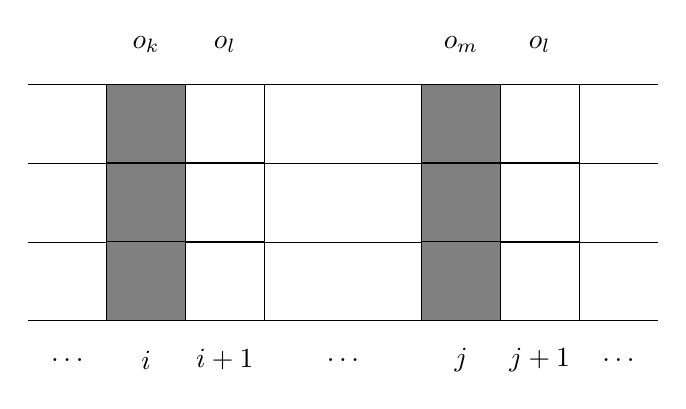
\begin{tikzpicture}
  \tikzstyle{box} = [draw=black, minimum width=10mm, minimum height=10mm];
  \tikzstyle{gray_box}  = [box, fill=gray];
  \tikzstyle{white_box} = [box];


  \draw[very thin] (-1.5, -0.5) -- (6.5, -0.5);
  \draw[very thin] (-1.5, 0.5)  -- (6.5, 0.5);
  \draw[very thin] (-1.5, 1.5)  -- (6.5, 1.5);
  \draw[very thin] (-1.5, 2.5)  -- (6.5, 2.5);

  \node[gray_box]  at (0, 0) {};
  \node[white_box] at (1, 0) {};
  \node[gray_box]  at (4, 0) {};
  \node[white_box] at (5, 0) {};

  \node[gray_box]  at (0, 1) {};
  \node[white_box] at (1, 1) {};
  \node[gray_box]  at (4, 1) {};
  \node[white_box] at (5, 1) {};

  \node[gray_box]  at (0, 2) {};
  \node[white_box] at (1, 2) {};
  \node[gray_box]  at (4, 2) {};
  \node[white_box] at (5, 2) {};

  \node at (0, 3) {$o_k$};
  \node at (1, 3) {$o_l$};
  \node at (4, 3) {$o_m$};
  \node at (5, 3) {$o_l$};

  \node at (-1, -1) { $\dots$};
  \node at (0, -1)  { $i$};
  \node at (1, -1)  { $i+1$};
  \node at (2.5, -1)  { $\dots$};
  \node at (4, -1)  { $j$};
  \node at (5, -1)  { $j+1$};
  \node at (6, -1)  { $\dots$};
\end{tikzpicture}
%%% Local Variables:
%%% mode: latex
%%% TeX-master: "../master"
%%% End:

  \caption{Computing the full forward table from the partial table. The gray
    boxes indicate columns filled during the when computing the table for the
    compressed sequence. The white columns needs to be computed in less than
    $O(N^2)$ time per column.}
  \label{fig:full-forward-table}
\end{figure}

Unfortunately no solution to this problem has been found. Hence, the posterior
decoding cannot be speeded up by exploiting repetitions in the observed
sequence. The running time of computing the posterior decoding path is then
$O(M N^3 + TN^2)$, which is assymptotically worse than the classical posterior
decoding algorithm that runs in $O(TN^2)$. Note though that the alphabet size
$M$ typically is small, so it is expected that the assymptotic running times of
the two algorithms in practice are comparable.

\section{Subsequence Posterior Decoding}

In the last section it was discussed that the posterior decoding for a sequence
cannot be done assymptotically faster using the byte-pair compression. However,
if only parts of the posterior decoding path are needed instead of the entire
path, a speedup may be obtained.

For subsequence posterior decoding not only an input sequence $Y_{1:T}$ and a
model $\lambda$ is given as input, but also two indexes $i,j \in
[1:T], i \ge j$. Instead of returning the posterior decoding path $X_{1:T}$ the
subpath $X_{i:j}$ is returned.

Recall from section (?)\fxwarning{Provide reference} that the columns of the
forward and backward tables of the compressed sequence are a subset of columns
in the tables of the uncompressed sequence. Furthermore, recall that a column
may be computed using the column emmediately to the left or right for the
forward and backward algorithms respectively. Using this, the forward and
backward tables $\alpha$ and $\beta$ of the subsequence $Y_{i:j}$ may be found
using existing columns from the forward and backward tables of the compressed
sequence. An example of this situation is illustrated in
figure~\ref{fig:subsequence-posterior}.

\begin{figure}
  \centering
  \tikzsetnextfilename{subsequence_posterior}
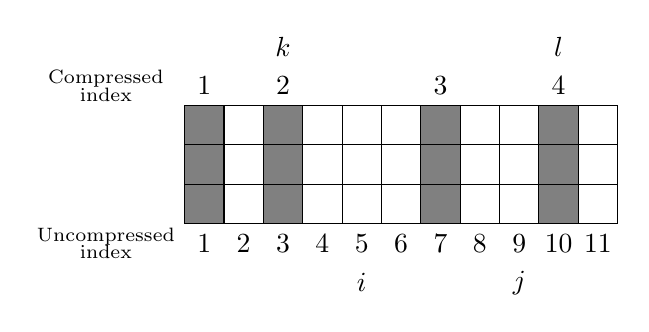
\begin{tikzpicture}
  [scale=0.5]
  \tikzstyle{box} = [draw=black, minimum width=5mm, minimum height=5mm];
  \tikzstyle{gray_box}  = [box, fill=gray];
  \tikzstyle{white_box} = [box];


  \node at (2, 4) {$k$};
  \node at (9, 4) {$l$};

  \node[gray_box]  at (0, 0) {};
  \node[gray_box]  at (0, 1) {};
  \node[gray_box]  at (0, 2) {};

  \node[white_box]  at (1, 0) {};
  \node[white_box]  at (1, 1) {};
  \node[white_box]  at (1, 2) {};

  \node[gray_box]  at (2, 0) {};
  \node[gray_box]  at (2, 1) {};
  \node[gray_box]  at (2, 2) {};

  \node[white_box]  at (3, 0) {};
  \node[white_box]  at (3, 1) {};
  \node[white_box]  at (3, 2) {};

  \node[white_box]  at (4, 0) {};
  \node[white_box]  at (4, 1) {};
  \node[white_box]  at (4, 2) {};

  \node[white_box]  at (5, 0) {};
  \node[white_box]  at (5, 1) {};
  \node[white_box]  at (5, 2) {};

  \node[gray_box]  at (6, 0) {};
  \node[gray_box]  at (6, 1) {};
  \node[gray_box]  at (6, 2) {};

  \node[white_box]  at (7, 0) {};
  \node[white_box]  at (7, 1) {};
  \node[white_box]  at (7, 2) {};

  \node[white_box]  at (8, 0) {};
  \node[white_box]  at (8, 1) {};
  \node[white_box]  at (8, 2) {};

  \node[gray_box]  at (9, 0) {};
  \node[gray_box]  at (9, 1) {};
  \node[gray_box]  at (9, 2) {};

  \node[white_box]  at (10, 0) {};
  \node[white_box]  at (10, 1) {};
  \node[white_box]  at (10, 2) {};

  \node[align=center] at (-2.5, 3) {\scriptsize Compressed \\[-2mm] \scriptsize index};

  \node at (0, 3) {1};
  \node at (2, 3) {2};
  \node at (6, 3) {3};
  \node at (9, 3) {4};

  \node[align=center] at (-2.5, -1) {\scriptsize Uncompressed \\[-2mm] \scriptsize index};

  \node at (0, -1) {1};
  \node at (1, -1) {2};
  \node at (2, -1) {3};
  \node at (3, -1) {4};
  \node at (4, -1) {5};
  \node at (5, -1) {6};
  \node at (6, -1) {7};
  \node at (7, -1) {8};
  \node at (8, -1) {9};
  \node at (9, -1) {10};
  \node at (10, -1) {11};

  \node at (4, -2) {$i$};
  \node at (8, -2) {$j$};

\end{tikzpicture}
%%% Local Variables:
%%% mode: latex
%%% TeX-master: "../master"
%%% End:

  \caption{Illustration of the computation of the forward (or backward) table
    for a substring of the uncompressed sequence given by indices $i$ to $j$,
    given that the forward table for the compressed sequence, shown in grey,
    has been computed in advance.}
  \label{fig:subsequence-posterior}
\end{figure}

Assume that the forward table $\alpha'$ and the backward table $\beta'$ for the
compressed sequence has been computed. This is shown as grey columns.

To compute $\alpha$ and $\beta$ for $Y_{i:j}$, the computed column at some index
$k$ to the left of index $i$ may be used as a starting point for the forward
computation. In this example that is column 2 when using indexes from the
compressed sequence. Likewise, some column $l$ with $l$ being to the right of
$j$ can be used as a starting point for the computation of the backward
table.

To find the indicies $k$ and $l$ for the uncompressed sequence and the
corresponding indicies $k'$ and $l'$ for the compressed sequence, a sorted
mapping \texttt{orig\_index2comp\_index} from uncompressed indices to
compressed indices is created. In this example the map would consist of the
mappings $1 \rightarrow 1, 3 \rightarrow 2, 7 \rightarrow 3$ and
$10 \rightarrow 4$. To find the index $k$, a binary search is performed on the
map to find the largest key less than $i$. The value corresponding to this key
is the index to the column in the forward table of the compressed sequence that
should be used as starting point for the forward computation of the
uncompressed sequence.

The mapping is computed as follows. First, another mapping
\texttt{symbol2length} from each symbol in the new alphabet $\mathcal{O'}$ to
its original length is created. This may be done iteratively by inserting first
inserting each original symbol $o_1, \dots, o_M \in \mathcal{O}$ with length 1
into the map. Next, $o_{M+1}, o_{M+2}, \dots, o_{M'} \in \mathcal{O'}$ is
inserted in the specified order. As each new symbol $o_k \in \mathcal{O'}$ is
created using two existing symbols $o_i$ and $o_j$ the length of $o_k$ can be
computed by using the map to get the the lengths of $o_i$ and $o_j$ and add
these.

Next, \texttt{orig\_index2comp\_index} is computed by scanning through the
compressed sequence one symbol at a time while incrementing the corresponding
index in the uncompressed sequence by using the map of lengths.

Now the first column of $\alpha$ is easily found by finding $k'$ using a binary
search as just discussed. Similarly the last column of $\beta$ can be
found. The only thing missing for the computation is the substring for which
$\alpha$ and $\beta$ should be computed.

A simple way of doing this would be decompressing $Y_{k':l'}'$ to obtain
$Y_{k:l}$, then compute columns corresponding to this subsequence and
afterwards remove columns $[k, i)$ and $(l, n]$. Decompressing $Y_{k':l'}'$
entirely might be inefficient though. If the compressed sequence $Y_{1:T'}'$ is
much compressed, i.e.\ $T' \ll T$, the length of $Y_{k:l}$ will be much larger
than $Y_{i:j}$. In the worst case of $T' = 1$, the decompression would result
in the uncompressed sequence $Y_{1:T}$. Then and the algorithm will spend a lot
of time computing columns and throwing these away afterwards. Hence, the
decompression needs to be made smarter.

Observe that only the symbols from index $[i,j]$ needs to be from the orignal
alphabet $\mathcal{O}$. The symbols from $[k, i)$ and $(j, l]$ may be from the
new alphabet, since each column in the these parts of $\alpha$ and $\beta$ are
not needed for the posterior decoding computation. Hence, when decompressing
$Y_{k':l'}'$ symbols that correspond to uncompressed symbols in the interval
$[k, i)$ should not be decompressed and left as compressed symbols. Likewise,
symbols corresponding to the interval $(j, l]$ should not be
decompressed. Symbols corresponding to uncompressed symbols that overlap
$[i, j]$ should be decompressed. The partially decompressed sequence $Z$ will
then contain some symbols from $\mathcal{O'}$ a the beginning, then some
symbols from $\mathcal{O}$ in the middle, being the symbols $Y_{i:j}$, and the
some symbols from $\mathcal{O'}$ in the end.

An algorithm for doing this takes as input a compressed sequence $Y'$ and the
indicies $i, j, k, l, k'$ and $l'$. The symbols of substring $Y_{k':l'}'$ is
pushed to a stack $Y^S$, such that $Y_{l'}'$ is at the bottom and $Y_{k'}'$ at
the top. The algorithm may be implemented iteratively, by popping symbols one
by one from $Y^S$, while the corresponding uncompressed index into the
uncompressed sequence $Y$ is maintained by using the \texttt{symbol2length}
map. When a symbol $c$ that overlap $[i, j]$ is encountered $c$ is either
appended to $Z$ if $c \in \mathcal{O}$ or it is split into a pair and added to
the front of $Y$, such that the left symbol of that pair will be removed in the
next iteration. The first time a symbol $c \in \mathcal{O}$ overlaps $[i, j]$
is encountered, the index of that symbol in $Z$ is saved, as it must be used
later for computing the posterior decoding. If $c$ overlaps $[k, l]$ it is
appended to $Z$. In case there is no overlap between $c$ and $[k, l]$ nothing
is done, i.e.\ $c$ is thrown away. Pseudo code for this algorithm is given in
algorithm~\ref{alg:decompress}.

\begin{algorithm}
  \caption{Partially decompress the compressed sequence.}
  \label{alg:decompress}
  \begin{algorithmic}[1]
    \Procedure{decompress\_substring}{$Y, i, j, k, l, k', l'$}
        \State{String $Z \gets $ nil}
        \State{Stack $Y^S \gets $ nil}
        \State{Push $Y_{l'}, \dots, Y_{k'}$ to $Y^S$}
        \State{start\_index $\gets$ nil}
        \State{index $\gets k - (\text{symbol2length[}Y^S\text{.top()]} - 1)$}
        \While{$Y^S$ is not empty}
            \State{$c \gets Y^S\text{.pop()}$}
            \State{next\_index $\gets$ index + symbol2length[$c$]}
            \If{$(\text{index} \le i \land \text{next\_index} > i) \lor
                 (\text{index} > i \land \text{index} \le j)$}
                \If{$c \in \mathcal{O}$} \Comment{$c$ overlaps $[i, j]$}
                    \State{$Z$.append($c$)}
                    \If{start\_index is nil}
                        \State{start\_index $\gets$ $Z$.size() $- 1$}
                    \EndIf{}
                \Else{}
                    \State{$c_l, c_r \gets$ get\_pair($c$)}
                    \State{Push $c_r, c_l$ to $Y^S$}
                    \State{\textbf{continue}}
                \EndIf{}
            \ElsIf{$(\text{index} \le k \land \text{next\_index} > k) \lor
                       (\text{index} > k \land \text{index} \le l)$}
                \State{$Z$.append($c$)} \Comment{$c$ overlaps $[k, l]$}
            \EndIf{}
            \State{index $\gets$ next\_index}
        \EndWhile{}
        \State{\Return{$Z$, start\_index}}
    \EndProcedure{}
\end{algorithmic}
\end{algorithm}

In the previous paragraphs the start columns from $\alpha'$ and $\beta'$, that
is the columns at index $k'$ and $l'$ respectively, have been found. There are
used as the first column of the forward table $\alpha$ and the last column of
the backward table $\beta$. Furthermore, the substring $Z$ for which to compute
the the tables have been found. To complete the substring posterior decoding
algorithm equation~\eqref{eq:6} is used.

\subsection{Running Time}
\label{sec:running-time-2}

As described the computation of the forward and backward tables, $\alpha$ and
$\beta$, for the uncompressed subsequence depends on the tables $\alpha'$ and
$\beta'$ of the compressed sequence. If preprocessing/compression of the input
string $Y$ is not included it takes time $O(M' N^3 + N^2 T')$ to
compute. Performing the binary search on the map to find the indicies
$k, l, k'$ and $l'$ takes $O(\log T')$ time. Decompressing the subsequence
takes time proportional to the length of the decompressed subsequence, that is
$O(j - i + \delta)$, where $\delta$ is the number of symbols in the
intervals $[k, i)$ and $(j, l]$.  Computing $\alpha$ and $\beta$ takes time
$O(M N^3 + N^2 (j - i + \delta))$.  Summing this up a running time of
$O(M' N^3 + N^2 T' + N^2 (j - i + \delta))$ is obtained.



%%% Local Variables:
%%% mode: latex
%%% TeX-master: "master"
%%% End:
